% MSc dissertation example file, February 2022
%
% Leave one of the documentclass lines uncommented to match your degree.
% You may remove the logo option if it causes problems.
% Do not change any other options.
% \documentclass[logo,msc,adi]{infthesis}     % Adv Design Inf
% \documentclass[logo,msc,ai]{infthesis}      % AI
% \documentclass[logo,msc,cogsci]{infthesis}  % Cognitive Sci
% \documentclass[logo,msc,cs]{infthesis}      % Computer Sci
% \documentclass[logo,msc,cyber]{infthesis}   % Cyber Sec
% \documentclass[logo,msc,datasci]{infthesis} % Data Sci
% \documentclass[logo,msc,di]{infthesis}      % Design Inf
% \documentclass[logo,msc,dsti]{infthesis}    % Data Sci TI
% \documentclass[logo,msc,inf]{infthesis}     % Informatics
\documentclass[logo,msc]{infthesis}           % degree unspecified, do not change except to add your degree
%%%%%%%%%%%%%%%%%%%%%%%%
% Understand any problems and seek approval before assuming it's ok to remove ugcheck.
\usepackage{msccheck}

% Include any packages you need below, but don't include any that change the page
% layout or style of the dissertation. By including the ugcheck package above,
% you should catch most accidental changes of page layout though.

\usepackage{microtype} % recommended, but you can remove if it causes problems
\usepackage{caption}
\usepackage{subcaption}
\usepackage{url}
\usepackage{graphicx}

\begin{document}
\begin{preliminary}

\title{OpenTTDLab: A framework for repeatable, Replicable, \& Reproducible experiments using OpenTTD}

\author{Michal Charemza}

\date{\today}

\abstract{
OpenTTD is an open source real time strategy (RTS) business simulation game based on the 1994 game Transport Tycoon Deluxe. In spite of being designed as a recreational game, OpenTTD has been the focus of a number of academic studies. However, these studies have problems regarding the repeatability, replicability, \& reproducibility of their experiments. This paper summarises the problems, presents a framework that allows OpenTTD to be used in a way to avoid these problems in future research, and uses this framework to find some initial results showing that OpenTTD can be used in supply chain research.
}

\maketitle

\newenvironment{ethics}
   {\begin{frontenv}{Research Ethics Approval}{\LARGE}}
   {\end{frontenv}\newpage}

\begin{ethics}
This project was planned in accordance with the Informatics Research
Ethics policy. It did not involve any aspects that required approval
from the Informatics Research Ethics committee.

\standarddeclaration
\end{ethics}


\begin{acknowledgements}
TODO Acknowledge the other contributors to OpenTTDLab (including to the pre-forked code), stating clearly what they did.
\end{acknowledgements}


\tableofcontents
\end{preliminary}


\chapter{Introduction}

OpenTTD \cite{openttd} is an open source real time strategy (RTS) simulation game. The aim of the game is to successfully run a business by constructing networks of roads, railways, airports and ports, along with their respective vehicles, trains, planes and ships, in order to transport people and goods in exchange for money. OpenTTD is played on a simulated landscape as can be seen in Figure \ref{fig:openttd}.

\begin{figure}[h]
\centering
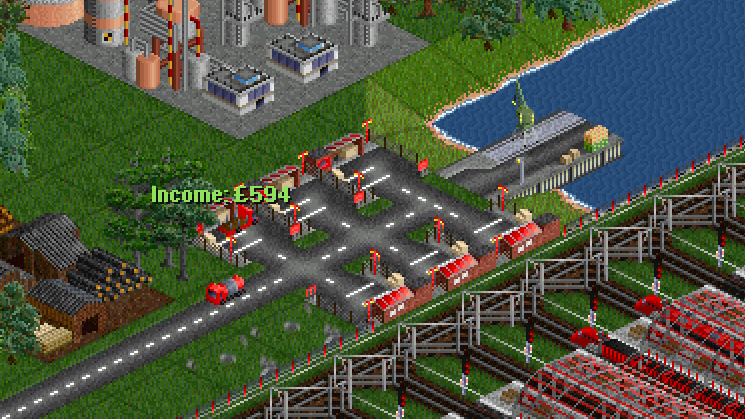
\includegraphics[width=\columnwidth]{assets/openttd-screenshot.png}
\caption{A small section of an OpenTTD (version 12.2) game at the moment when income is received for delivering goods by road. Also shown is part of a railway network, a port for ships, an oil refinery, and a sawmill.}
\label{fig:openttd}
\end{figure}


OpenTTD was created as a game for recreation. However, it is remarkably flexible: it has been successfully used as a tool to research artificial intelligence (AI) and machine learning (ML) algorithms \cite{wisniewski2011artificial, rios2009trains, bijlsma2014evolving}, scalability and mobile applications \cite{jiang2018mirroring}, and as a teaching aid \cite{HansenMuprhie2018}. It allows a single player to play in a non competitive world building mode, multiple human players playing cooperatively or competitively, and allows so-called custom AI-players that each control a company via code not part of the OpenTTD, but part of extensions to it written in the Squirrel language.

Using OpenTTD as a tool for research is the focus of this project, and specifically its features for repeatable, replicable, \& reproducible research.

\section{History of simulation games in research}

\begin{itemize}

\begin{item}
\cite{jackson1959learning} first business simulation game, US Air force MONOPOLOGS pretend to be inventory managers
\end{item}

\begin{item}
\cite{meijer2009organisation} - Studying supply chains using gaming simulation
\end{item}

\begin{item}
\cite{mayer2009gaming} - Defines simulation game as a game "experi(m)ent(i)al, rule-based, interactive environments, where players learn by taking actions and by experiencing their effects through feedback mechanisms that are deliberately built into and around the game"
\end{item}

\begin{item}
\cite{raghothama2013review} war gaming roots, policy analysis, business simulation games, studies on human cognition and behavior, training and pedagogical tools

Main point: simulation games particular suited for transportation research in general, and supply chain specifically because it's an emergent property
\end{item}

\end{itemize}

OpenTTD is part of a wider class of games: simulation games. Simulation games have been frequently used in various fields to explore scenarios in an effort to inform policies. PUT IN LIST.

Attention is usually paid to how realistic these games are. For example, \cite{raghothama2013review} summarises how well a number of games, including OpenTTD, how well the games model the real world. It's worth noting that while the economic model of OpenTTD is not realistic, \cite{raghothama2013review} classes some aspects of the transportation model as realistic, albeit without justification.

MORE

There have been calls \cite{dalle2012reproducibility}, cited

In terms of the existing, they don't follow

\section{Repeatability, Replicatability, \& Reproducibility}

The terms repeatability, replicability, and reproducibility unfortunately do not historically have universally agreed meanings \cite{plesser_reproducibility_2018}. To add to the confusion, the ACM have swapped their definitions reproducibility and replicability \cite{association_for_computing_machiner_new_2020}. For the avoidance of doubt, I use the ACM's definitions that are current as of October 2023 \cite{association_for_computing_machiner_artifact_2020}. For some results of an experiment conducted by a team of authors, where some computer-based artefacts were created to conduct these, these can be summarised as

\begin{description}
\item[Repeatability] The authors can obtain the results again, using the same artefacts.
\item[Reproducibility] A different team can obtain the results, using the original authors' artefacts.
\item[Replicability] A different team can obtain the results, without using any of the original authors' artefacts.
\end{description}

The strongest of these these, replicability, does not require a full re-implementation of all artifacts used in the research, but only those created by the original team. In OpenTTD terms, if an author writes a custom AI that is used in experiments, only that AI would need to be implemented by another team to replicate the research. OpenTTD itself would not need to be re-implemented in order for experiments to satisfy the definition of replicability.

Beyond just supplying definitions, the ACM also provide a system of 5 badges, as seen in Figure \ref{fig:acm_badges}. These can be applied to published research to incentivise research authors to make it so their research is reproducible and replicable by other teams. Other similar systems of badges are available.

\begin{figure}
     \centering
     \begin{subfigure}[b]{0.3\columnwidth}
         \centering
         
\includegraphics[width=\textwidth]{assets/artifacts_available.jpg}
         \caption{Artifacts available}
         \label{fig:y equals x}
     \end{subfigure}
     \hfill
     \begin{subfigure}[b]{0.3\columnwidth}
         \centering
         
\includegraphics[width=\textwidth]{assets/artifacts_evaluated_functional.jpg}
         \caption{Artifacts evaluated functional}
         \label{fig:three sin x}
     \end{subfigure}
     \hfill
     \begin{subfigure}[b]{0.3\columnwidth}
         \centering
         
\includegraphics[width=\textwidth]{assets/artifacts_evaluated_reusable.jpg}
         \caption{Artifacts evaluated reusable}
         \label{fig:five over x}
     \end{subfigure}
    \par\bigskip
     \begin{subfigure}[b]{0.3\columnwidth}
         \centering
         
\includegraphics[width=\textwidth]{assets/results_reproduced.jpg}
         \caption{Results reproduced}
         \label{fig:five over x}
     \end{subfigure}
     \begin{subfigure}[b]{0.3\columnwidth}
         \centering
         
\includegraphics[width=\textwidth]{assets/results_replicated.jpg}
         \caption{Results replicated  safd }
         \label{fig:five over x}
     \end{subfigure}
        \caption{The ACM system of badges for reproducble research}
        \label{fig:acm_badges}
\end{figure}

It is my hope that the framework presented here will make it more likely that research using OpenTTD will be not only repeatable, reproducible and replicable, but also more likely that upon publication, given all of these badges. 

\section{Review of research using OpenTTD}

From the found published research using OpenTTD, in my opinion there is yet to be a single case that couldn't offer significant improvements in at least one of its repeatability, replicability or replicability.

\subsection{Repeatability}

Repeatability should be the easiest of the 3Rs to achieve, especially with computer based simulation. However, much of the existing research using OpenTTD uses a low number of repeated experiments, with little or no statistical analysis, suggesting that it was not straightforward. The experiments of \cite{wisniewski2011artificial} were run just 3 times for example. The experiments in \cite{rios2009trains} were run 14 times, but not even for the same amount of in-game time.

\subsection{Reproducibility}

For reproducibility the author-supplied artifacts must be clear and available. There were references to modified OpenTTD in \cite{wisniewski2011artificial}, but the modified versions does not seem to be available. Potentially the authors could be contacted to supply their own artefacts, but this is not ideal, nor offers a strong guarantee that the artefacts supplied were exactly as they were that generated the results.

Also, the version of OpenTTD is not mentioned

The seeds of each experiements were also not supplied.

\subsection{Replicability}

This is the most difficult to judge without actually attempting to do it, and it is what.

However, if an experiemnt isn't even reproducible, it is even more difficult to replicate it.

\chapter{Existing features of OpenTTD}

\section{Review of OpenTTD command line options and configuration}
OpenTTD as of version 13.4 has over X command line options and Y configuration options that allow the player to customise how it behaves when playing. The ones that are particularly applicable to a  for repeatable, reproducible, and replicable research are reviewed below.

\subsection{Command line options}

\begin{description}
\item[-G \textless seed\textgreater] Allows the specification of the seed that initialises the random number generator that controls the pseudo random aspects of the game. For example, OpenTTD can auto generate landscapes. With the same seed (along with other configuration) one generation will be the same as the next
\item[-g] Starts a game immediately, rather than requiring the user to click through a introductory menu 
\item[-vnull:ticks=\textless number of ticks\textgreater] Puts the same into a "null" video mode that does not display the playing area on screen, and exits the game after a set number of \emph{ticks}. A tick is equal to approximately 1/Y of a day in game time.
\end{description}

The specification of the random seed should mean that OpenTTD affords exact repeatability and reproducibility when running as a simulation using only AI players. This means that it should be possible to make it straightfoward for to make results exactly reproducible, going beyond the requirements for ACM's badges on that front.

\subsection{Configuration options}

\begin{description}
\item[{fast\_forward\_speed\_limit} = \textless limit\textgreater] Limits the ticks per second the limit, which has a hard coded maximum in the game of 50000

\item[{[ai\_players]}] Allows the specification of which player are human and which are AI, and when they start playing.

\item[autosave = monthly|daily|other CHECK]

\item[keep\_all\_autosave]  A boolean value that allows all autosaves to be kept for further analysis
\end{description}


\section{The save game format}

OpenTTD saves its data in a custom binary format - its so-called savegame format. OpenTTD offers an extremely basic tool for extracting some data from this format. However, a separate Python based tool is available to extract data from save games

\chapter{The framework}

The framework has two audiences. The first audience is an experimenter looking to conduct experiments with an AI, be it their own, or others, or a combination. The second is someone looking to reproduce or replicate another team's results. As such it contains separate instructions for both of these audiences.

\subsection{The experimenting team}

It takes the command line options in code, the various options of OpenTTD, and outputs two things:

\begin{itemize}
\item The results of the experiments - these are as Python variable, which allows the persistance of the results to be chosen by the experimenter. For example, in a basic CSV format.
\item The metadata of the experiments: the version of OpenTTD, the version of the framework itself, any commend line options, and all configuration, highlighting the configuration the differs from the defaults for that version of OpenTTD
\end{itemize}

\subsection{The reproducing or replicating team}

This leads to the second audience. The framework contains instructions to follow for a separate team trying to reproduce or replicate the experiments of the first team. These instructions mean that the first team can role-play as a reproducer or replicator, and test themselves how straightforward it is to reproduce the experiments, and judge for themselves if it is possible that their results be reproduced, and their research be awarded the badges of Figure \ref{fig:acm_badges}.

The replicability of results would be more difficult to judge - the author's artefacts cannot be used in this case, which means that if a team want to role play, they have to recreate their own artefacts, without reference to their original. The system here at least means that the "boilerplate" is handled, and this can be focused on.

\chapter{Results from using the framework relating to supply chains}

The framework has been used to extract how the bank balance from OpenTTD change over time for a company controlled by the TrainAI as in \label{fig:value-over-time}. The 

\begin{itemize}
  \item This has been created using a non-modified version of OpenTTD 13.1.
  \item The exact random seeds are shown
  \item There are 50 experiments run
  \item Each is run for the same amount of in game time
\end{itemize}

The output of the seeds used, all settings, OpenTTD version, without modification, should make the experiments repeatable, reproducible, and ideally replicable. Thus it is an improvement in these terms over many of the results reviewed in section 4.

A limitation of the framework is that the AI version used doesn't seem to have a version.

\begin{figure}[h]
\centering
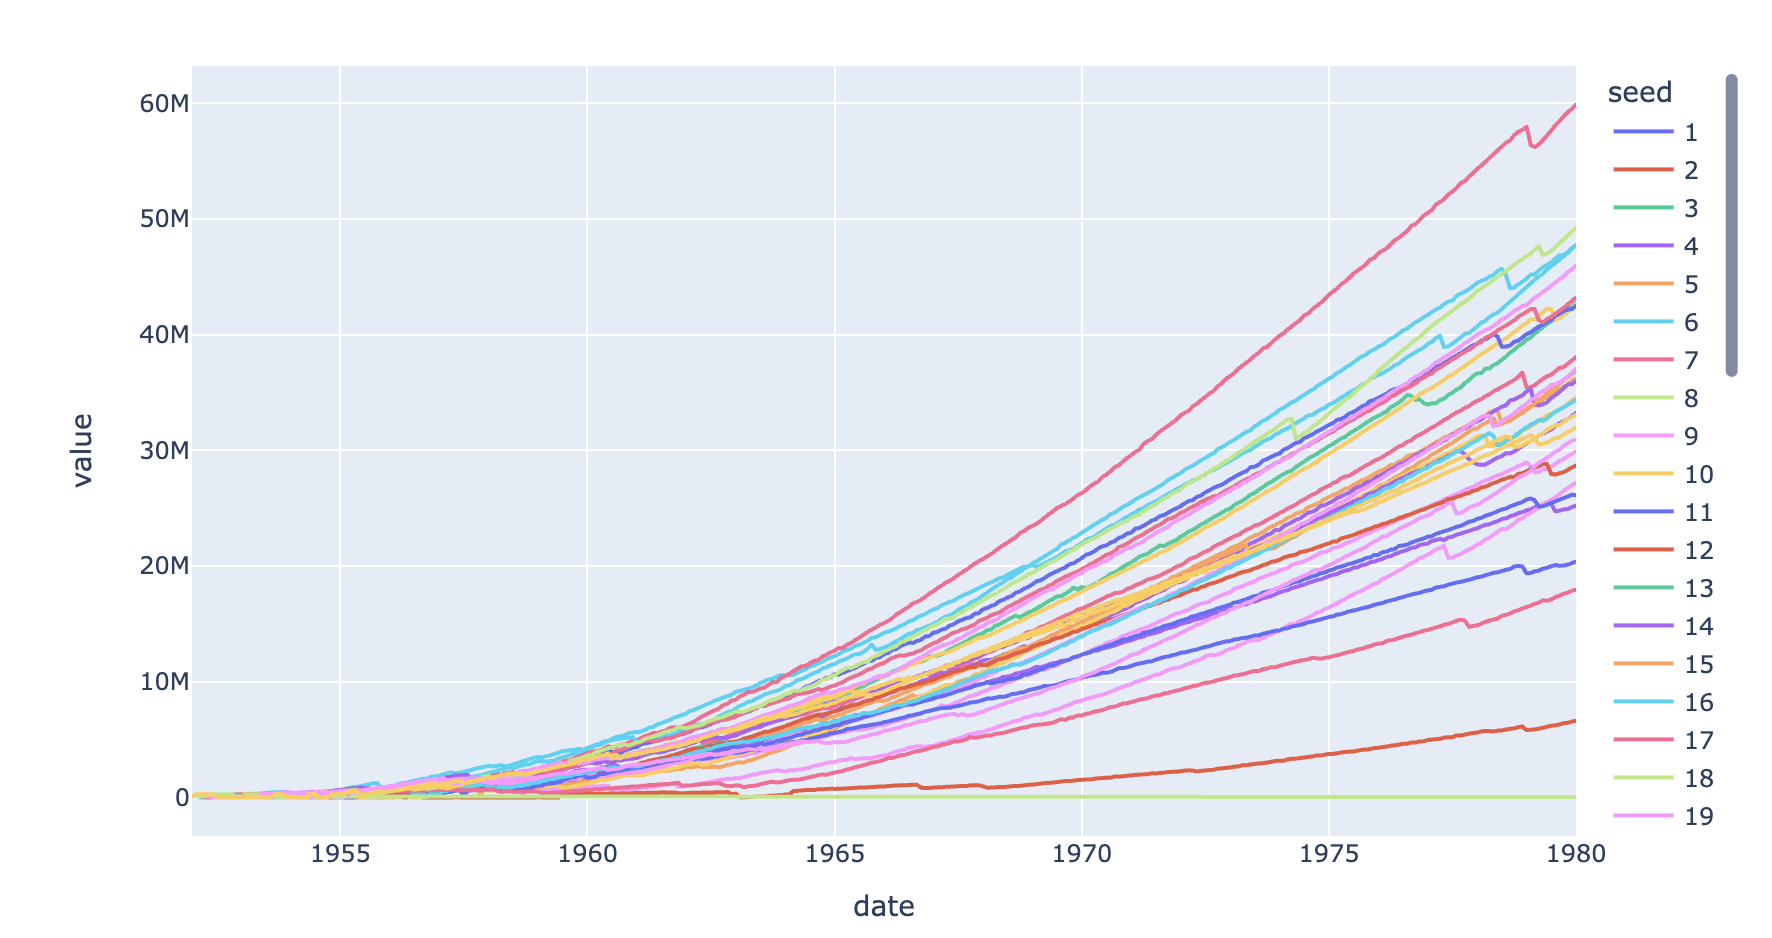
\includegraphics[width=\columnwidth]{assets/value-over-time.png}
\caption{A chart showing the balance over for 50 experiments}
\label{fig:value-over-time}
\end{figure}

\chapter{Conclusion}

The framework presented here allows experiments to be conducted with OpenTTD in a manner that is repeatable and reproducible. Reproducibility is up to the author's descriptions of the artefacts they created - they must be sufficient to recreate the artefacts, and so beyond the scope of the framework here. However, it should at least ease issues due to creating a similar enough experimental setup.

The exception are the version of the AI used - these do not appear to be versioned. However, potentially it could report on some sort of hash of the code of the AI.



\bibliographystyle{plain}
\bibliography{mybibfile}


% You may delete everything from \appendix up to \end{document} if you don't need it.
\appendix

\chapter{First appendix}

\section{First section}

Any appendices, including any required ethics information, should be included
after the references.

Markers do not have to consider appendices. Make sure that your contributions
are made clear in the main body of the dissertation (within the page limit).


\end{document}
